

\chapter{SHIM DIF for WiFi}

\section{Introduction}

In this chapter we will stipulate the Specification of the Shim DIF over WiFi. This DIF will only provide support for RINA DIFs. Given that a RINA DIF expects a RINA API as the lower API, the purpose of a Shim DIF is to create as thin a veneer as possible over a legacy protocol (WiFi) to allow a RINA DIF to use it without modification.  The goal is not to make legacy protocols provide full support for RINA and so the shim DIF should provide no more service or capability than the legacy protocol provides.

\npar

\begin{table}[H]
		\begin{center}
		\begin{tabular}{|lc|}
			\hline
				802.2 & LLC		\\ \hline
				802.11 & MAC		\\ \hline
				802.11 & PHY		\\
			\hline
		\end{tabular}
		\caption{Overview of WiFi protocol parts}
		\end{center}
\end{table}

WiFi consists of 3 main parts and the adaptor will try to span over all these. On top we have the 802.2 LLC layer, below that is the 802.11 MAC layer and finally we have the 802.11 physical layer. We must note that the LLC layer is an old protocol that has been reused for WiFi, it is not likely to be updated soon. The LLC layer is currently being used to differentiate between different higher level data packets. The MAC layer has been changed as recently as 2007 with 802.11e. It has several fields reserved for future use and could be changed later on. Finally, the physical layer is presented at the bottom of the WiFi scope. We instantly note that this changed quite often but provides no additional use towards the Shim DIF. The physical layer of WiFi is not within the scope of the Shim DIF. 

\npar

The Shim DIF over WiFi is not a fully functional DIF. This means that some limitations apply to this protocol:

\begin{itemize}
	\item Limited amount of flows due to the usage of the LLC header for flow differentiation (802.2 standard\citep{ieee8022std}).
	\item Only type 1 operation of LLC is useable, this means no Data State Vectors can be used
\end{itemize}

The reason why we can only use Type 1 operation is because the other types (2 \& 3) require constant ACKing of packets. These packets are then marked with ACK numbers, limited to 128 different values. This is considered too low in the current high bandwidth traffic that can occur. Thus only Type 1 operation, which has no ACKing, but also Data State vectors, can be used. Even with these restrictions the Shim DIF provides enough support at the bottom layer of the architecture that other DIFs can build further upon. The Shim DIF provides QoS-cubes, flow differentiation and other options such as fragmentation possibilities. The Shim DIF presents the WiFi stack towards upper layer DIFs as a DIF.

\section{Mapping of 802.11 MAC header}

In this section we will show how we will use WiFi. We will start the mapping from the 802.11 MAC layer. Here we focus on 802.11e, this IEEE standard from 2005 implements the most recent version of MAC. This includes the introduction of QoS, used later on in this specification. 

\npar

The fields in the 802.11 MAC header (shown in figure~\ref{fig:80211macframe}) that will be used are the Address Fields and Payload field.

\begin{figure}[H]
    \centering
    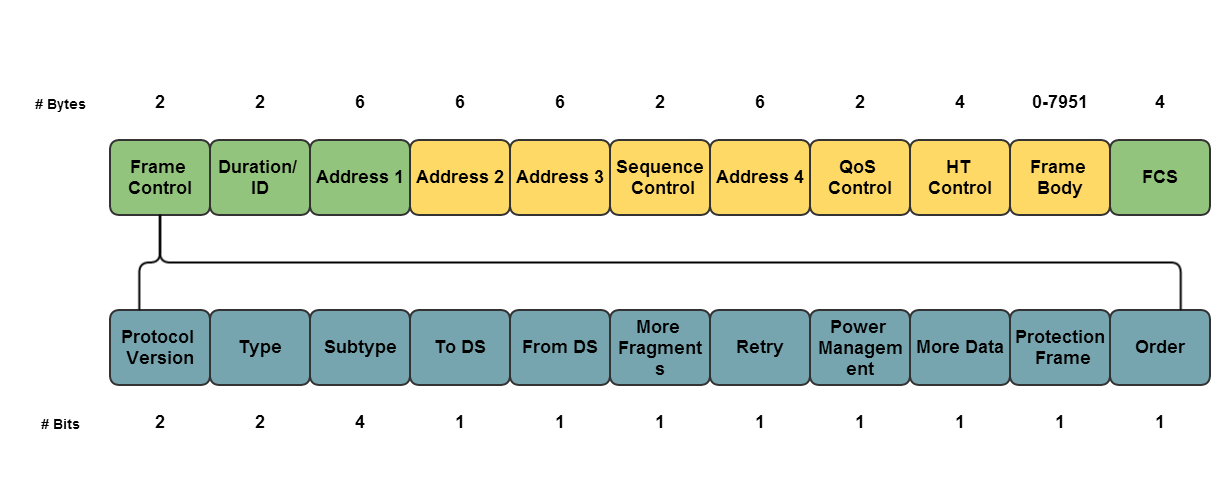
\includegraphics[width=1\textwidth]{figures/80211macframe}
    \caption{802.11 MAC frame} 
    \label{fig:80211macframe}
\end{figure}

These 4 address fields will be used according to the 802.11 MAC standard~\citep{ieee80211std}. This means the following address fields will be mapped:

\begin{description}

\item[Address fields] The MAC addresses used to identify shim IPC Processes to.
\\


%table for address fields
\begin{table}[H]
%\begin{adjustbox}{width=\textwidth,keepaspectratio}
	\begin{center}
		\begin{tabulary}{1.0\textwidth}{|L|L|L|L|L|L|L|}
			\hline
				\textbf{Network Type} & \textbf{To DS bit} & \textbf{From DS bit} & \nohyphens{\textbf{Address 1}} & \nohyphens{\textbf{Address 2}} & \nohyphens{\textbf{Address 3}} & \nohyphens{\textbf{Address 4}} \\ \hline
				IBSS (ad hoc) & 0 & 0 & DA & SA & BSSID & \emph{N/A} \\ \hline
				BSS (infrastructure) & 0 & 1 & DA & BSSID & SA & \emph{N/A} \\ \hline
				BSS (infrastructure) & 1 & 0 & BSSID & SA & DA & \emph{N/A} \\ \hline
				WDS & 1 & 1 & RA & TA & DA & SA \\
			\hline
		\end{tabulary}
		\caption[Overview of Address Fields]{Overview of Address Fields\protect\footnotemark}
	\end{center}
%\end{adjustbox}
\end{table}

\footnotetext{Only DA and SA are used in the Shim IPC Process}

%end table address fields
\begin{description}
	\item[Destination Address (DA)] The Shim IPC process address corresponding to the WiFi interface that the destination Shim IPC Process is bound to.
	\item[Source Address (SA)] The Shim IPC process address corresponding to the WiFi interface of this Shim IPC Process.
\end{description}

Note that these address fields are static in the Shim and are determined according to the values in the Frame Control field, further details shall not be provided for this as this is provided in the IEEE standard\citep{ieee80211std}.  

\item[Frame Body] This is the SDU it received from the upper DIF. An SDU can be fragmented as 802.11 supports fragmented payload\footnote{More Fragments subfield in the Frame Control field}

\end{description} 

The DIF name is the SSID (Service Set Identifier). This name is provided by periodical advertisement in a beacon frame.


\section{Mapping of 802.2 LLC header}

\begin{table}[H]
		\begin{center}
		\begin{tabular}{|c|c|c|c|}
			\hline
				\textbf{DSAP address} & \textbf{SSAP address} & \textbf{Control} & \textbf{Information} \\ \hline
				8 bits & 8 bits & 8 or 16 bits & M*8 bits \\ 
			\hline
		\end{tabular}
		\caption{802.2 LLC PDU format}
		\end{center}
\end{table}

The 802.2 LLC header will primarily be used for differentiating between different connections for the upper layer DIF. For further information and documentation on this standard we refer to the IEEE document~\citep{ieee8022std}.

\subsection{SAP addressing}
\label{ssec:sap-addressing}

SAPs will be used to distinguish between different connections, the current address assignments for SAP can be found in the table below. These SAP assignments only have to be unique within their scope and are not required to be globally unique. Every SAP is a CEP-id, during flow allocation they are mapped to a port-id. This port-id forms the boundary between the 0-DIF (Shim DIF) and the 1-DIF.

\npar

\begin{table}[H]
	\begin{center}
		\begin{tabular}{|c|c|c|c|c|c|c|c|c|c|c|c|c|c|c|c|}
			%\hline
				\multicolumn{8}{|l|}{$<$ Least significant bit} & \multicolumn{8}{l|}{$<$ Least significant bit} \\
				\hline
				I/G & D\textsuperscript{ISO} & D & D & D & D & D & D & C/R & S\textsuperscript{ISO} & S & S & S & S & S & S \\
				\hline
				\multicolumn{16}{l}{} \\
				\multicolumn{1}{l}{I/G} & \multicolumn{1}{l}{0} & \multicolumn{1}{l}{=} & \multicolumn{13}{l}{Individual DSAP} \\
				\multicolumn{1}{l}{I/G} & \multicolumn{1}{l}{1} & \multicolumn{1}{l}{=} & \multicolumn{13}{l}{Group DSAP} \\
				\multicolumn{1}{l}{C/R} & \multicolumn{1}{l}{0} & \multicolumn{1}{l}{=} & \multicolumn{13}{l}{Command} \\
				\multicolumn{1}{l}{C/R} & \multicolumn{1}{l}{1} & \multicolumn{1}{l}{=} & \multicolumn{13}{l}{Response} \\
				\multicolumn{1}{l}{I/G} &  \multicolumn{2}{l}{\texttt{0 DD DDDD}} & \multicolumn{1}{l}{=} & \multicolumn{12}{l}{DSAP address} \\
				\multicolumn{1}{l}{C/R} &  \multicolumn{2}{l}{\texttt{0 SS SSSS}} & \multicolumn{1}{l}{=} & \multicolumn{12}{l}{SSAP address} \\
				\multicolumn{1}{l}{I/G} &  \multicolumn{2}{l}{\texttt{1 DD DDDD}} & \multicolumn{1}{l}{=} & \multicolumn{12}{l}{Reserved for ISO definition} \\
				\multicolumn{1}{l}{C/R} &  \multicolumn{2}{l}{\texttt{1 SS SSSS}} & \multicolumn{1}{l}{=} & \multicolumn{12}{l}{Reserved for ISO definition} \\
				
				
			%\hline
		\end{tabular}
		\caption{SAP Address Assignment}
	\end{center}
\end{table}

\npar

This leaves 6 bits per address field free to choose. The least significant bit is always on the left, this means that when presenting these addresses as hex. We will only use individual SAPs and discard the Command/Response bit due to not having Data State Vectors available. The second least significant bit will also be left 0, due to the ISO definition3. This means we can only use \{0, 4, 8, C\} for our last hex symbol. This leaves the following possibilities free to choose from: 0x\{XY\}. With X = \{0, 1, 2, 3, 4, 5, 6, 7, 8, 9, A, B, C, D, E, F\} and Y = \{0, 4, 8, C\}. In total, 64 SAP addresses can be used within the Shim DIF.



\subsection{DSAP address field}

The Destination Service Access Point will be used to identify the flow on the destination IPC Process. For correct mapping on addressing we op to currently store a mapping between application-naming and connection address locally.

\subsection{SSAP address field}

The Source Service Access Point will be used for to identify the flow on the current IPC Process. For correct mapping on addressing we op to currently store a mapping between application-naming and connection address locally.

\section{Use of Address Resolution Protocol}
\label{sec:arp}

Because the RINA Flow Allocator is unavailable at this low level, we opt to reuse ARP for this WiFi Shim DIF. ARP will be used to map an application-naming (1-DIF) to the address of a Shim IPC Process (0-DIF). ARP can normally be used to map a network address of variable, unlimited length to a link layer address of any length. However, the most used implementation is the IPv4 ARP implementation \citep{arp1998}.
\\
Below is the ARP frame represented by this IPv4 ARP implementation. Any further references to ARP will imply the use of this frame, which is RFC826 compliant\footnote{\url{http://tools.ietf.org/html/rfc826}}.


\begin{table}[H]
	\begin{center}
		\begin{tabular}{|c|c|}
			\hline
				\textbf{Bit 0-7} & \textbf{Bit 8-15} \\ \hline
				\multicolumn{2}{|c|}{Hardware type} \\ \hline
				\multicolumn{2}{|c|}{Protocol ethertype} \\ \hline
				Hardware address byte length & Protocol address byte length \\ \hline
				\multicolumn{2}{|c|}{Opcode (ARP Request or ARP Response)} \\ \hline
				\multicolumn{2}{|c|}{Hardware address sender (n bytes)} \\ \hline
				\multicolumn{2}{|c|}{Protocol address sender (m bytes)} \\ \hline
				\multicolumn{2}{|c|}{Hardware address target (if known) (n bytes)} \\ \hline
				\multicolumn{2}{|c|}{Protocol address target (m bytes)} \\ \hline
		\end{tabular}
		\caption{ARP frame format (RFC826 compliant)}
	\end{center}
\end{table}

\npar

In the chart below we show how ARP is used in the Shim DIF. Locally an ARP table is kept with entries which map Shim IPC Process Addresses (MAC addresses) to Application names. When data transfer is required, the Shim IPC Process sends out an ARP request to find the Shim IPC Process Address which corresponds to the application name of the destination. The local ARP cache is queried and the corresponding Shim IPC Process responds with an ARP response with the Shim IPC Process Address.

\npar

\begin{figure}[H]
    \centering
    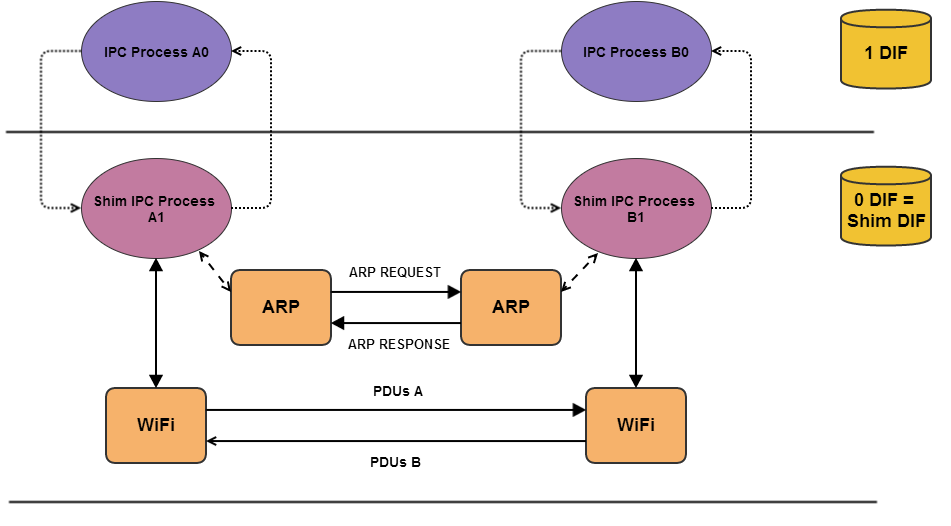
\includegraphics[width=1\textwidth]{figures/arp_example}
    \caption{ARP example} 
    \label{fig:arp_example}
\end{figure}

\npar

ARP has a 1 byte length field for the network protocol address. For the Shim DIF we will be using ASCII coding, this leaves us with a maximum of 255 characters for the length of the network protocol address. Due to RINA specifications, a name can consist of 4 parts, which will be encoded in this network protocol address. The encoding we use is bencoding. It is defined in the specification\footnote{\url{https://wiki.theory.org/BitTorrentSpecification\#Bencoding}} with the bittorrent protocol.

\npar

\begin{table}[H]
	\begin{center}
		\begin{tabular}{|l|l|}
			\hline
				Process name & Echo-IPC-Process  \\ \hline
				Process instance & 1 \\ \hline
				Entity name & Data \\ \hline
				Entity instance & 1 \\ \hline
		\end{tabular}
		\caption{Application-Naming information}
	\end{center}
\end{table}

\npar

Encoded this becomes: ``16:echo-IPC-Process1:14:Data1:1''. Note that these are all strings. As an alternative we can also use a synonym for the application name. A synonym for this is the name of the Application Process instance with a default Application Entity instance. 
\\
Since we need to send the source and destination application name, but we only have one network protocol length field, we choose the longest application name. The other, shorter application name is then filled with padding (zero bytes, 0x00) which are removed by the receiving IPC Process. This causes some overhead, but this overhead stays very small because these ARP frames only need to be sent during the flow allocation phase.


\section{Service Definition}

In this section the different QoS-cubes that are supported will be addressed.

\subsection{QoS-cubes supported}

The WiFi protocol supports several QoS-cubes, they are a combination of following possibilities. 
\npar
Because QoS-cubes are separated in 4 categories we will offer 4 QoS-cubes. The categories are the following: voice, video, background, best effort. This gives us the following QoS cubes:

\begin{table}[H]
		\begin{center}
		\begin{tabular}{|l|l|}
			\hline
				ID 										& 		1 \\ \hline
				Name 									&			Voice \\ \hline
				Average bandwidth 		&			Depends on 802.11 physical standard \\ \hline
				Average SDU bandwidth 									&			Depends on 802.11 physical standard										 \\ \hline
				Peak bandwidth-duration 									&		Depends on 802.11 physical standard											 \\ \hline
				Peak SDU bandwidth-duration 									&			Depends on 802.11 physical standard										 \\ \hline
				Burst period 									&			Depends on 802.11 physical standard										 \\ \hline
				Burst duration 									&		Depends on 802.11 physical standard											 \\ \hline
				Undetected bit error rate 									&			Depends on 802.11 physical standard										 \\ \hline
				Partial delivery 									&			Allowed										 \\ \hline
				Order 									&				Depends on 802.11 physical standard									 \\ \hline
				Max allowable gap in SDUs 				&				Depends on 802.11 physical standard									 \\ \hline
				Delay 									&			Depends on 802-11 physical	standard									 \\ \hline
				Jitter 									&			Depends on 802-11 physical standard										 \\ \hline
				Ack policy							&			Depends on kernel settings				\\ \hline
		\end{tabular}
		\caption{QoS cube for traffic categorized as Voice}
		\end{center}
\end{table}

\npar

\begin{table}[H]
	\begin{center}
		\begin{tabular}{|l|l|}
			\hline
				ID & 2  \\ \hline
				Name & Video \\ \hline
		\end{tabular}
		\caption{QoS cube for traffic categorized as Video}
	\end{center}
\end{table}

\npar

\begin{table}[H]
	\begin{center}
		\begin{tabular}{|l|l|}
			\hline
				ID & 3  \\ \hline
				Name & Background \\ \hline
		\end{tabular}
		\caption{QoS cube for traffic categorized as Background}
	\end{center}
\end{table}

\npar

\begin{table}[H]
	\begin{center}
		\begin{tabular}{|l|l|}
			\hline
				ID & 4  \\ \hline
				Name & Best\_effort  \\ \hline
		\end{tabular}
		\caption{QoS cube for traffic categorized as Best effort}
	\end{center}
\end{table}

Note that we do not provide full tables as below the Name section these are all the same, dependent on the physical standard over which communication is done. 

\section{Configuration}

Every Shim IPC Process is assigned to a WiFi interface. Before the Shim DIF can become operational it needs a basic amount of information. This information is comprised of:

\subsection{Shim IPC Process info}

The WiFi device address is the Shim IPC Process address and the SSID is the DIF name. This SSID is broadcasted periodically as a beacon frame. This info also includes other information such as: WEP-key, WPA, \ldots.

\subsection{Port-id to CEP-id directory}

The WiFi Shim DIF has different flows available through the use of CEP-ids. In the subsection~\ref{ssec:sap-addressing} about SAP mapping we saw that 64 connections can be differentiated. Each one has a 1-byte long address. This SAP address is a Connection EndPoint-Identifier (CEP-id). The CEP-id is locally mapped on the port-id. The port-id is a transfer point on the boundary between the 1-DIF and the 0-DIF. 

\subsection{Application to SAP mapping}

Since no explicit flow allocation is possible, it is currently not possible to choose the SAP addresses freely. They will be mapped to applications locally in a file. This file contains a mapping for application naming info to SAP addresses. When communication is set up the Shim IPC Process retrieves the right SAP address from this file based on the requesting application. Or the Shim IPC Process delivers to the correct application process based on the SAP address. 

\section{Bootstrapping}

Upon creation the Shim IPC Process communicates with the OS to address the traffic from WiFi towards the Shim IPC Process. This traffic must be part of the same DIF (SSID), the MAC address must be the same as the interface the Shim IPC process is bound to. Finally the SAP must be used by the Shim DIF. When these conditions are fulfilled we assume that all traffic is RINA traffic and should be handled by the Shim IPC Process.

\section{Application (un)registration}

If an Application Process (AP) registers with the Shim IPC Process. Upon registration of the application, the Shim IPC Process's directory adds an item. This item maps the AP name to the MAC address. The MAC address is bound to the Shim IPC process. Finally when an AP un-registers the Shim IPC Process removes the entry in the ARP cache. If future queries of the application name are triggered, they will be ignored if the entry is not present in the cache.

\section{Enrollment}

All members with an interface active in the same SSID are assumed to be in the same Shim DIF. When a new member enlists in this Service Set it is enrolled in the Shim DIF. 

\section{WiFi Shim IPC Process Definition}
\label{sec:wifi_shim_ipc_proc_def}

The Shim IPC process over WiFi assumes the following API from ARP:

\begin{description}
	\item[arpAdd(netaddress).submit] Adds a mapping of network address, in RINA the application name, to the MAC interface in the ARP table of the interface. In essence this maps the application process to the Shim IPC process address. The function returns: 'success' when the mapping was added, 'failure' when it was not. 
	\item[arpRemove(netaddress).submit] This is the inverse of the action of the previous function. It removes a mapping of the application name to the MAC address in the ARP table. If this entry is removed it returns: 'success', otherwise 'failure' is returned.
	\item[arpMapping(netaddress).submit] Requests ARP for a mapping of a network address to a MAC address. When the mapping is found, arpMapping(netaddress, hwaddress).deliver is called.
\end{description}

These 3 functions are provided by ARP.

\npar

The Shim IPC process over WiFi also assumes the following functions from API regarding the CEP-id to port-id mapping.

\begin{description}
	\item[ci-piAdd(CEP-id,Port-id).submit] This adds a mapping between a CEP-id and a Port-id. If this entry is added it returns: ``success'', otherwise ``failure'' is returned.
	\item[ci-piRemove(CEP-id,Port-id).submit] This removes a mapping between a CEP-id and a Port-id. Since this is a 1(Port-id)-to-N(CEP-id) mapping it is allowed that one of the function variables is void. In case the CEP-id is void, all CEP-ids corresponding to the Port-id will be removed, in case the Port-id is empty, only one CEP-id to Port-id entry will be removed. If this entry is removed it returns: ``success'', otherwise ``failure'' is returned.
	\item[sapMapping(CEP-id,Port-id,Application-naming).submit] Requests the Shim IPC Process to look in the provided table to find a mapping between the CEP-id and the Application-naming. If successful this calls ci-piAdd(CEP-id,Port-id) and consequently calls a positive sapMapping.deliver(+). If the unsuccessful a negative sapMapping.deliver(-) is called and no mapping is added to the CEP-id to Port-id directory. Note that this function always requires a Port-id and either a CEP-id (receiving Shim IPC Process) or Application-naming (sending Shim IPC Process). 
\end{description}

\npar

Port-ids are linked to CEP-ids and are tristate variables. The 3 states of a port-id are the following:

\begin{description}
	\item[NULL] The port-id is unusable in this state
	\item[PENDING-SP] This state of the port-id can originate from two possibilities. The application process has initiated the flow allocation, requested sapMapping and is idle in the PENDING-SAP state until it receives an sapMapping.deliver. The other option is that it has received a request to create a flow and is currently waiting for the sapMapping.submit function to finish, it stays in the PENDING-SAP until it receives sapMapping.deliver.
	\item[PENDING-ARP] This state of the port-id can originate from 2 possibilities. The port-id has received the sapMapping.deliver(+) function and the arpMapping.query has been called. The port is idle in the PENDING-ARP state until it receives the arpMapping.deliver. The other possibility is that the request to create a flow has delivered the sapMapping.deliver(+) and is waiting for the allocateResponse.submit to finish the flow allocation.
	\item[ALLOCATED] This state indicates that the flow has been allocated and the port-id can be used to read/write data to/from.
\end{description}

\npar

Below are all the possible functions for the Shim IPC process and finally a state diagram with said functions is presented.

\subsection{applicationRegister(naming-info).submit}
\subsubsection{When invoked}
This primitive is invoked to register an application on top of the shim IPC process.  The application becomes available in the shim DIF. This primitive has to be invoked before all other functions. ARP does not differentiate between client/server, which means every application has to be available in the ARP table, even clients.
\subsubsection{Action upon receipt}
The naming-info is transformed into a single string (application-name), with the method described in segment~\ref{sec:arp}. arpAdd(application-name).submit is called. If successful, a mapping of the application name to the hardware address of the device is added in the ARP table of the interface. The other primitives become usable. If it failed, they are not and an error is generated.


\subsection{applicationUnregister(naming-info).submit}
\subsubsection{When invoked}
This primitive is invoked to unregister an application on top of the shim IPC process. This unregisters the application in the shim DIF. No other primitives can be invoked until applicationRegister(naming-info).submit is called again. 
\subsubsection{Action upon receipt}
The naming-info is transformed into a single string (application-name), with the method described in section~\ref{sec:arp}. arpRemove(application-name).submit is called. If successful, the mapping of the application name to the hardware address of the device is removed from the ARP table of the device. If it fails, an error is generated.


\subsection{allocateRequest(naming-info).submit}
\subsubsection{When invoked}
This primitive is invoked by a source application to request a new flow. Naming-info consists of the destination upper layer IPC Process name $<$AP name, AE name$>$ (AP-name if there is a single Shim-DIF; AP-ApplicationEntity if there is more than one).
\subsubsection{Action upon receipt}
If there is already a flow established to the destination application (the port-id is in the ALLOCATED state), or there is a flow pending between the source and destination applications (the port-id is in the PENDING-SAP or PENDING-ARP state), a negative allocateResponse(reason).deliver is returned. If the port-id is in the NULL state, sapMapping(void, port-id,netaddr).submit is called. The port-id transitions to the PENDING-SAP state.


\subsection{allocateResponse(reason).submit}
\subsubsection{When invoked}
This primitive is invoked by the destination application in response to an allocateRequest(naming-info).deliver which is invoked by a positive sapMapping(reason).deliver.
\subsubsection{Action upon receipt}
If the port-id is not in the PENDING-ARP state, an error is generated. If it is and if the allocate response is positive a flow has been established for this port-id; any queued frames are delivered to the destination application. The port-id transitions to the ALLOCATED state. If it is negative the flow creation has failed and reason indicates the failure reason, all queued and future frames from this combination of source MAC address and source SAP are dropped. The port-id transitions to the NULL state.


\subsection{arpMapping(netaddr,hwaddr).deliver}
\subsubsection{When invoked}
This is invoked by the ARP protocol machine when a requested mapping becomes available in the ARP table. The Shim IPC process is supplied with the mapping of a network protocol address, application name in RINA, to a hardware address (hwaddr).
\subsubsection{Action upon receipt}
If the port-id is in the PENDING state, (there is an outstanding allocateRequest(naming-info).submit), an allocateResponse(reason).deliver is invoked, and the hardware address (MAC address) is stored for this flow.  In this case the port-id transitions to the ALLOCATED state. If the port-id is in the ALLOCATED state, nothing happens. If it is in any other state, an error is generated.

\subsection{sapMapping(CEP-id,Port-id,Naming-info).query}
\subsubsection{When invoked}
This can be invoked by the reception of a WiFi frame when the port-id is in the NULL state. The port-id transitions to the PENDING-SAP state and the Shim IPC process awaits the sapMapping(reason).deliver response. It can also be invoked by the allocateRequest.submit function. The port-id transitions to the PENDING-SAP state and awaits the sapMapping(reason).deliver response. If the port is in the ALLOCATED nothing happens.
\subsubsection{Action upon receipt}
When received, the locally stored ``SAP to naming-information'' database is queried. The response is the sapMapping(reason).deliver response.

\subsection{sapMapping(reason).deliver}
\subsubsection{When invoked}
This is invoked as a response to the sapMapping(CEP-id,Port-id,Naming-info).query after the ``SAP to naming-information'' has been inquired. 
\subsubsection{Action upon receipt}
If the naming-info is an error (sapMapping.deliver(-)) then the port-id transitions to the NULL state. If the information is genuine and the port-id was in the PENDING-SAP state then it transitions to the PENDING-ARP state. 

\subsection{Frame}
\subsubsection{When invoked}
When the port-id is in the ALLOCATED state, a frame may be sent.  Otherwise the frame is dropped.
\subsubsection{Action upon receipt}
When there is no flow for the combination of the MAC address that sent the frame and the receiving CEP-id, the sapMapping.query function is called and the port-id transitions to PENDING-SAP. If there is a flow for the sender's MAC address and the receiving CEP-id, and the port-id is in the ALLOCATED state, write.deliver is called. If it is in the PENDING-SAP or PENDING-ARP state, the packet is queued. If it is in the NULL state, the packet is dropped.


\subsection{read.submit}
\subsubsection{When invoked}
This is invoked by the application when it wants to read a SDU.
\subsubsection{Action upon receipt}
When the shim IPC process receives this primitive and the port-id is in the ALLOCATED state, it will create a frame, and pass it to the OS for delivery. It is assumed that neither fragmentation nor concatenation is performed by the shim IPC Process. This is done because the WiFi protocol provides the functions below the Shim-DIF. Therefore shim IPC Process uses a different frame for each SDU passed to it. If the port-id is not in the ALLOCATED state, an error is generated and the frame is dropped.


\subsection{write.submit}
\subsubsection{When invoked}
This is invoked by the application when it wants to send one or more SDUs. 
\subsubsection{Action upon receipt}
When the shim IPC process receives this primitive and the port-id is in the ALLOCATED state, it will create a frame, and pass it to the OS for delivery. It is assumed that neither fragmentation nor concatenation is performed by the shim IPC Process. This is done because the WiFi protocol provides the functions below the Shim-DIF. Therefore shim IPC Process uses a different frame for each SDU passed to it. If the port-id is not in the ALLOCATED state, an error is generated and the frame is dropped. 


\subsection{deallocate.submit}
\subsubsection{When invoked}
This service primitive is invoked by the application to discard all state regarding this flow. It is the responsibility of both the source and destination application to invoke this primitive. It is a local event.
\subsubsection{Action upon receipt}
When the shim IPC process receives this primitive, the port-id transitions to the NULL state.


\subsection{Corresponding state diagram}

A ``/'' represents a following, or void, function that is being called by the preceding function. 

\begin{figure}[H]
    \centering
    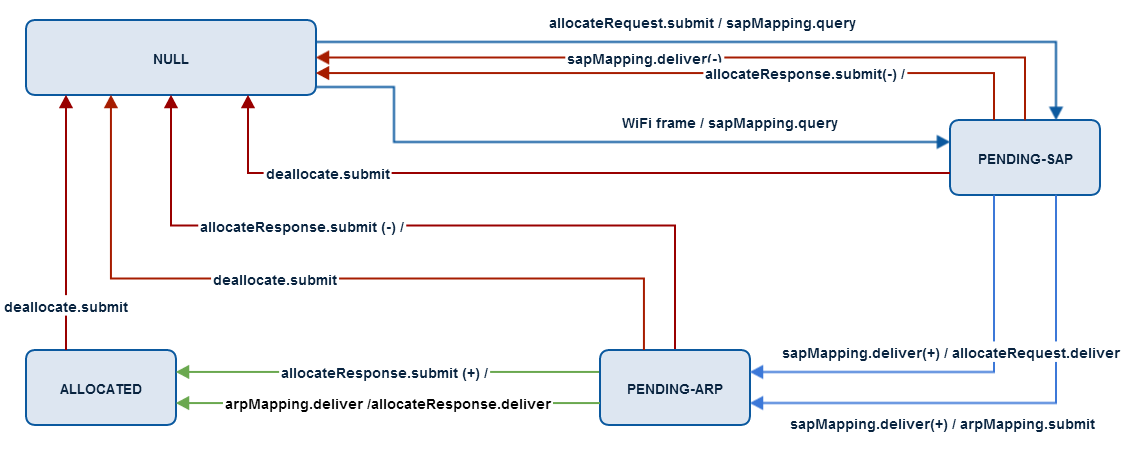
\includegraphics[height=0.6\textwidth, angle=270]{figures/state_diagram2}
    \caption{Corresponding state diagram} 
    \label{fig:state_diagram}
\end{figure}

